\clearpage

\subsection{EVL+STrace}
\label{sec:EVLPlusSTrace}

\NOTE{\emph{Solution expert:} Leila , \emph{Interviewer:} Thomas}

\NOTE{Preliminary text by Bernhard (by mistake)}

\subsubsection{Approach}
\label{sec:ApproachEVL}

The bx tool \emph{EVL+STrace} \cite{IST2018-Samimi} supports the synchronization of models on demand (no live synchronization) with the help of a persistently stored \emph{trace model} which stores links connecting source model elements and target model elements. The synchronizer receives the source model, the target model, and the trace model as inputs. After consistency has been established by a previous run of the synchronizer, both source and target models may have been modified. The synchronizer detects inconsistencies between the source model and the trace model, as well as between the trace model and the target model. Consistency is restored by propagating changes in both directions. Consistency restoration is performed interactively: The user is informed about consistency violations and is offered corresponding consistency repair actions. A repair action is performed only when it has been launched explicitly by the user.

\begin{figure}[tb!]
	\centering
	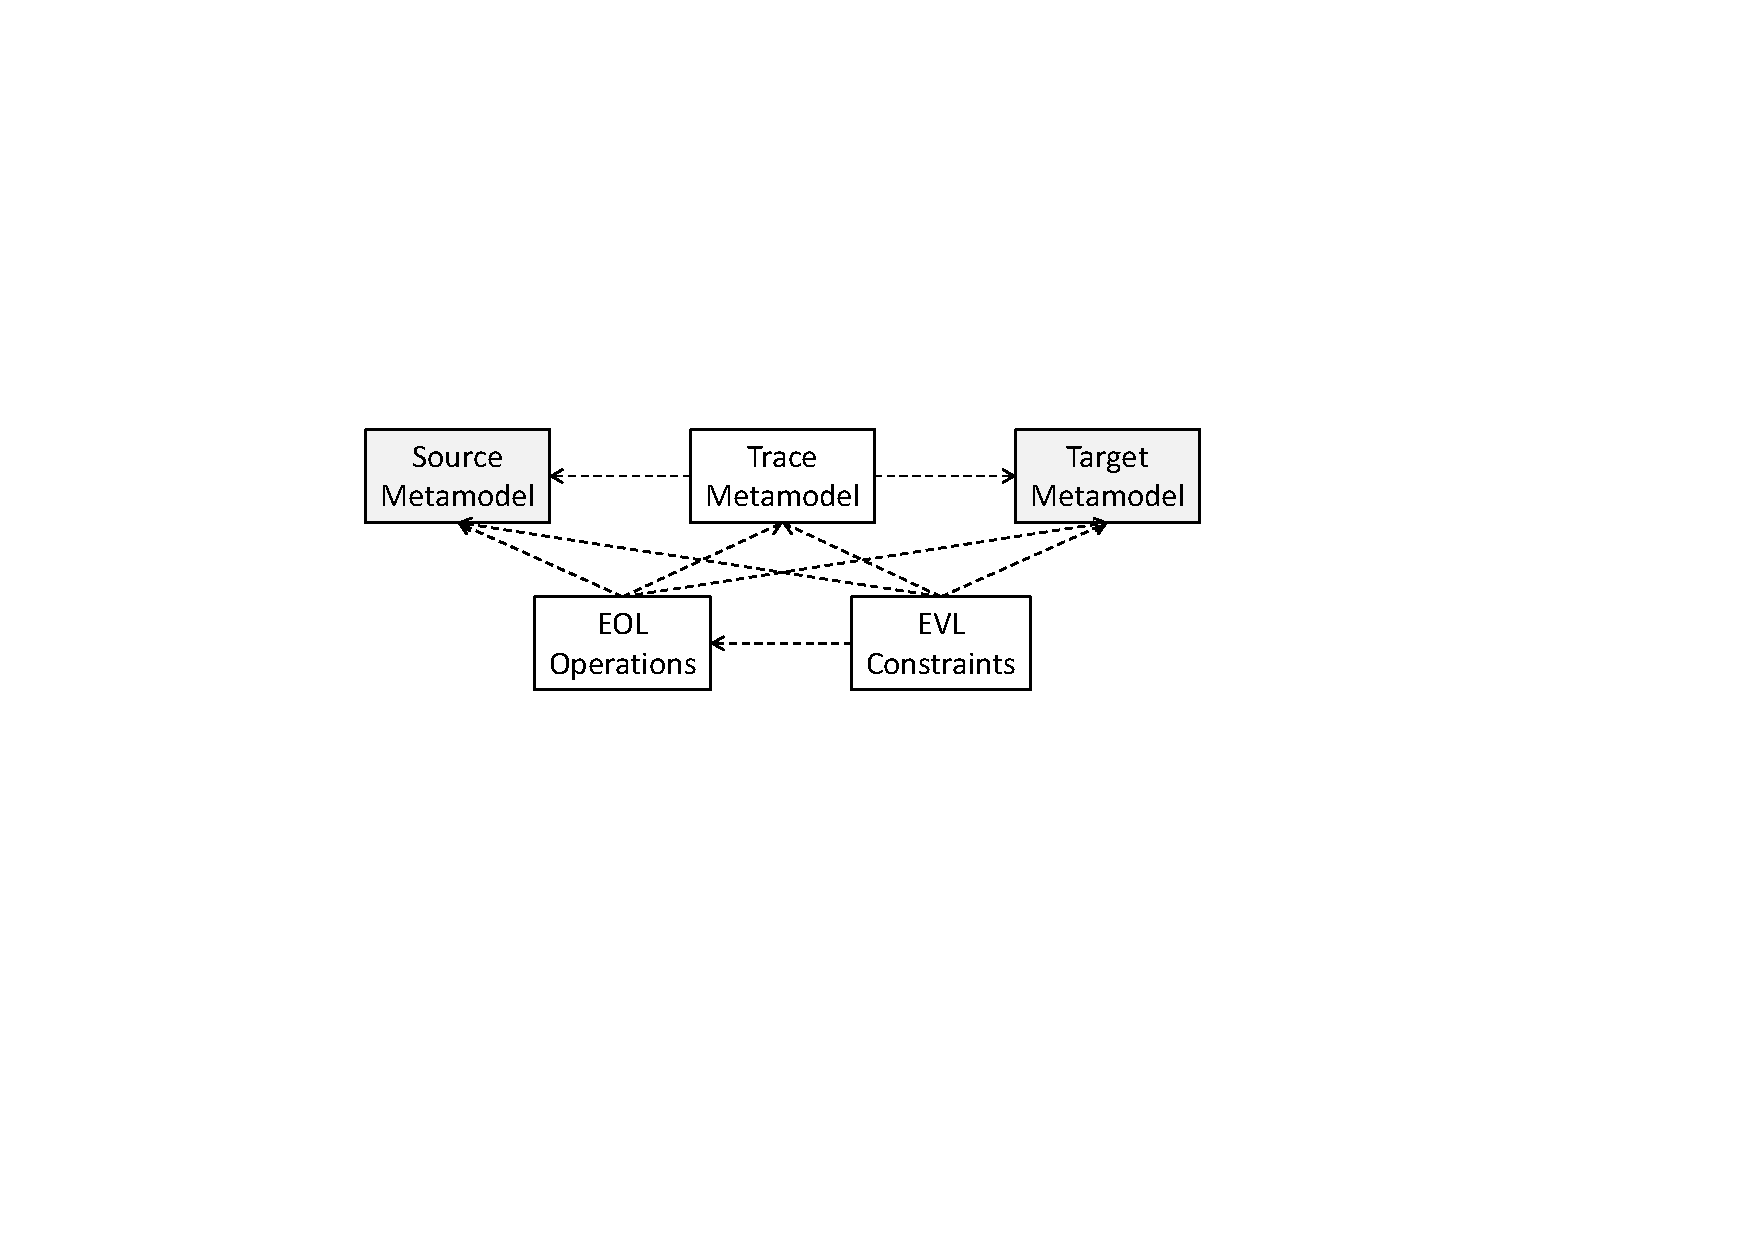
\includegraphics[width=0.8\columnwidth]{diagrams/EVLPlusSTraceArtefacts}
	\caption{Model artefacts and their dependencies in EVLPlusSTrace}
	\label{fig:evlartefacts}
\end{figure}

EVL+STrace is based on EMF as well as the \emph{Epsilon} framework \cite{epsilon}, which provides tool support for a variety of DSLs for model transformation. In EVL+STrace, a transformation definition consists of a trace metamodel, EOL operations, and EVL constraints. The \emph{trace metamodel} defines domain-specific types of links and link ends. Essentially, the trace metamodel is designed in such a way that a trace model contains copies of all relevant elements of source and target models, as well as links connecting these elements. By means of a rich trace model, it is possible to detect any category of changes to the participating models, including creation and deletion of objects and links, as well as modification of attribute values. The behavior of the synchronizer is defined by \emph{EOL operations}, i.e., operations for queries and updates written in the Epsilon Object Language, and \emph{EVL constraints}, i.e., constraints augmented with repair actions written in the Epsilon Validation Language. Each constraint is directed and checks an inconsistency between the trace model and one of the participating models which is caused by a change to this model. The corresponding repair action propagates this change to the trace model and the opposite model.

The artefacts making up the transformation definition may be generated partially from a \emph{weaving model}, which essentially includes the trace metamodel, augmented with behavioral properties being specified either by means of parameter values or by code fragments. The generator may create the trace metamodel completely, as well as large parts of EOL operations and EVL constraints, both of which may have to be refined and extended by the transformation developer. In this way, the transformation developer may save the effort of writing routine code for operations and constraints.

\subsubsection{Solution}
\label{sec:solutionEVL}

EVL+STrace participated in the Families to Persons benchmark at TTC 2017 \cite{Samimi-Dehkordi2017}. The synchronization concept underlying the Benchmarx framework differs from the approach implemented in EVL+STrace in two respects:

\begin{enumerate}
	\item The synchronization dialogues of the Benchmarx framework assume \emph{alternating changes}: Either an edit on the source model is propagated to the target model, which has not been modified concurrently, or propagation is performed in the opposite direction under analogous assumptions. In contrast, EVL+STrace allows for \emph{concurrent changes}.
	\item The Benchmarx framework assumes \emph{fully automatic change propagation} without any user interactions (which facilitates testing). In contrast, EVL+STrace supports \emph{fully interactive change propagation}.
\end{enumerate}

The first issue does not require special attention since EVL+STrace supports the more general case of concurrent changes; however, EVL+STrace will perform redundant checks (for changes on a model which is known to be unmodified) at runtime. We will deal with the second issue (automatic change propagation) at the end of this subsection. 

\begin{figure*}[tb!]
	\centering
	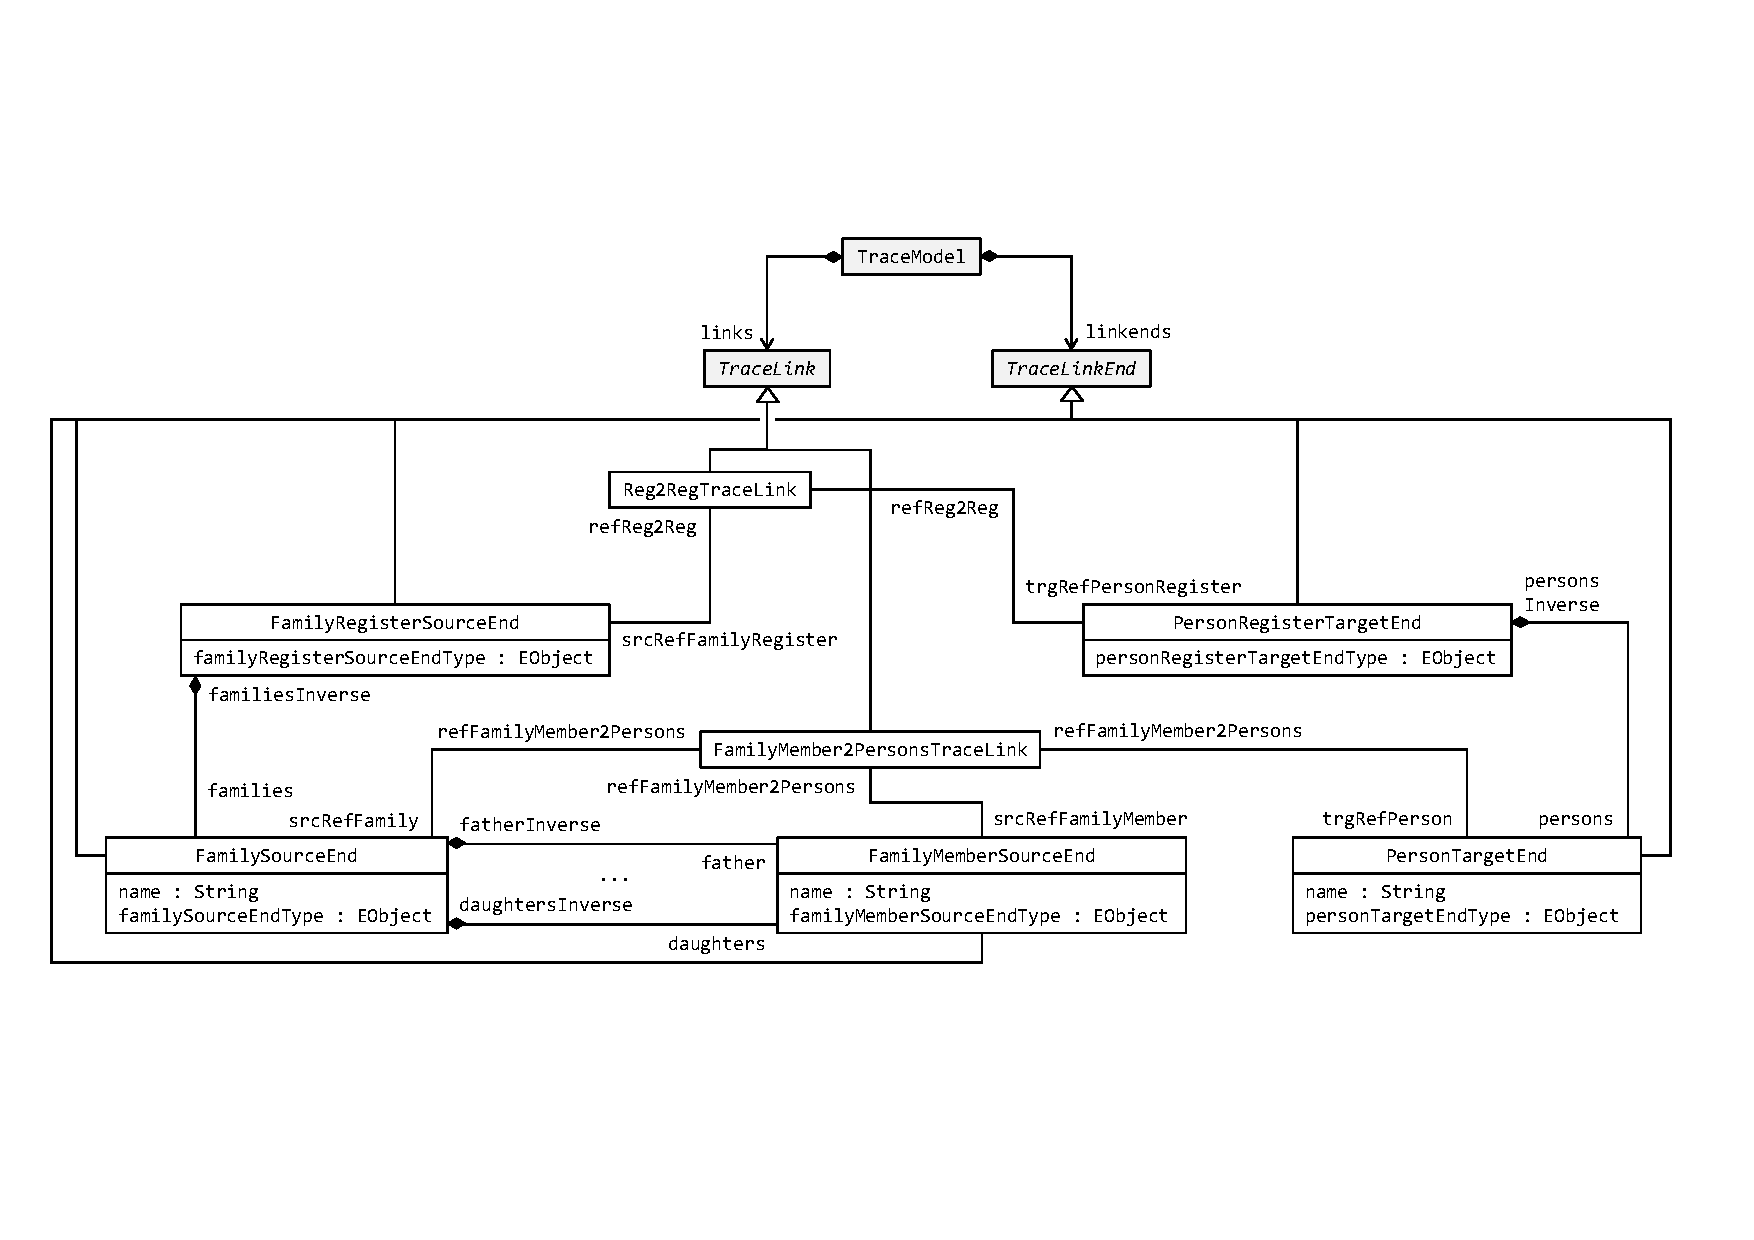
\includegraphics[width=\textwidth]{diagrams/EVLPlusSTraceMetamodel}
	\caption{Trace metamodel for Families to Persons (without multiplicities)}
	\label{fig:evltracemetamodel}
\end{figure*}

Figure~\ref{fig:evltracemetamodel} displays the \emph{trace metamodel} for the Families to Persons benchmark. Specific types of trace links and trace link ends are defined by subclassing built-in abstract superclasses \code{TraceLink} and \code{TraceLinkEnd}, respectively. Each \emph{trace link} references a set of trace link ends, which may be considered proxies of source or target model objects. \emph{Trace link ends} store links to source or target model objects with the help of attributes of type \code{EObject}. In addition, trace link ends may store attribute values and may be connected by links. In this way, the trace model may shadow the relevant parts of the source and target models. In the case of the Families to Persons benchmark, the trace metamodel defines two types of trace links for relating family and person registers as well as for relating family members along with their families with persons.


 
\lstdefinelanguage{evl}{
	morekeywords = {context,constraint,guard,not,self,and,check,message,fix,title,do,var,if,else,delete},
	morecomment=[l]{//},
	morecomment=[s]{/*}{*/}
}


\begin{lstlisting}[label={lst:evl}, float=*t, language=evl, caption={Example of an EVL constraint}]
context Families2Persons!FamilyMemberSourceEnd{
    guard: not self.isRemoved() and not self.refFamilyMember2Persons.endTypeIsRemoved()	
    constraint familyMemberRoleIsRelocated{
        check: not ((self.fatherInverse.isDefined() and not self.getEndType().fatherInverse.isDefined())
            or (self.motherInverse.isDefined() and not self.getEndType().motherInverse.isDefined())
            or (self.sonsInverse.isDefined() and not self.getEndType().sonsInverse.isDefined())
            or (self.daughtersInverse.isDefined() and not self.getEndType().daughtersInverse.isDefined()))		
        message: self+' role is changed'
        fix{
            title: 'Propagate the relocation for '+self
            do{
                var family= self.getEndType().getFamily();
                var person;
                if((self.fatherInverse.isDefined() or self.sonsInverse.isDefined()) and
                    self.getEndType().isFemale()){
                    person =insertFemale(family,self.getEndType());
                    person.birthday = self.refFamilyMember2Persons.trgRefPerson.getEndType().birthday;
                    var personTargetEnd = addPersonTargetEnd(person);
                    delete self.refFamilyMember2Persons.trgRefPerson.getEndType();
                    delete self.refFamilyMember2Persons.trgRefPerson;
                    self.refFamilyMember2Persons.trgRefPerson = personTargetEnd;
                }
                else 
                    if((self.motherInverse.isDefined() or self.daughtersInverse.isDefined()) and
                        self.getEndType().isMale()){
                        ...
                    }
            }
        }
    }
    ...
}
\end{lstlisting}

% This is the original code. The code above has been restricted to role changes only. It is not
% clear how the move to another family is handled. The guard of the constraint (stay in the same
% family) excludes a move. Then, the last operand of the check can be eliminated.
%\begin{lstlisting}[label={lst:evl}, float=*t, language=evl, caption={Example of an EVL constraint}]
%context Families2Persons!FamilyMemberSourceEnd{
%    guard: not self.isRemoved() and not self.refFamilyMember2Persons.endTypeIsRemoved()	
%    constraint familyMemberRoleIsRelocated{
%        guard: not self.getEndType().getFamily().isNew() and
%        self.getEndType().getFamily().getTraceLinkEnd()= self.getFamily()
%    check: not ((self.fatherInverse.isDefined() and not self.getEndType().fatherInverse.isDefined())
%        or (self.motherInverse.isDefined() and not self.getEndType().motherInverse.isDefined())
%        or (self.sonsInverse.isDefined() and not self.getEndType().sonsInverse.isDefined())
%        or (self.daughtersInverse.isDefined() and not self.getEndType().daughtersInverse.isDefined())
%        or (self.getEndType().getFamily().getTraceLinkEnd()<> self.getFamily()))		
%        message: self+' role is changed or\n'+self+' family ='+self.getFamily()+ 
%            'is changed to '+self.getEndType().getFamily()
%    fix{
%        title: 'Propagate the relocation for '+self
%    do{
%        var family= self.getEndType().getFamily();
%        var person;
%        if((self.fatherInverse.isDefined() or self.sonsInverse.isDefined()) and
%            self.getEndType().isFemale()){
%            person =insertFemale(family,self.getEndType());
%            person.birthday = self.refFamilyMember2Persons.trgRefPerson.getEndType().birthday;
%            var personTargetEnd = addPersonTargetEnd(person);
%            delete self.refFamilyMember2Persons.trgRefPerson.getEndType();
%            delete self.refFamilyMember2Persons.trgRefPerson;
%            self.refFamilyMember2Persons.trgRefPerson = personTargetEnd;
%        }
%        else 
%            if((self.motherInverse.isDefined() or self.daughtersInverse.isDefined()) and
%                 self.getEndType().isMale()){
%                        person = insertMale(family,self.getEndType());
%                        person.birthday = self.refFamilyMember2Persons.trgRefPerson.getEndType().birthday;
%                        var personTargetEnd = addPersonTargetEnd(person);				
%                        delete self.refFamilyMember2Persons.trgRefPerson.getEndType();
%                        delete self.refFamilyMember2Persons.trgRefPerson;
%                        self.refFamilyMember2Persons.trgRefPerson = personTargetEnd;}
%                        self.refFamilyMember2Persons.srcRefFamily = family.getTraceLinkEnd();	
%                        copySrc2Trg();
%
%}
%}
%}
%}
%...
%}
%\end{lstlisting}

Listing~\ref{lst:evl} gives a (slightly simplified) example of an \emph{EVL} constraint which deals with the relocation of a family member role. The \emph{context} in line~1 defines the set of objects on which the constraints inside the context declaration have to be evaluated (family member source ends in the trace model). The \emph{guard} in line~2 is shared by all constraints inside the context declaration and ensures that the member has not been removed (otherwise, the constraints are not applicable). The \emph{constraint declaration} starting in line~3 deals with the relocation of the role of a family member. The \emph{check} in lines~4--8 specifies the condition which has to be maintained: The family member must not have changed its role. The condition is checked by comparing links in the trace model against links in the families model. If a violation of this condition is detected (i.e., the role has changed), the \emph{message} in line~8 is used to inform the user about the violation. The proposed \emph{fix} is specified starting from line~9. The \emph{title} in line~10 is used to describe the fix to the user. The actual fix is contained in the \emph{do block} starting in line~11: The old person object is replaced with a new person object of the opposite gender to which the birthday of the old person object is copied.

As presented above, the EVL constraint will be repaired interactively. For automatic change propagation, the constraint definitions have to be modified by moving the do part into the check part and eliminating the message and the fix part. These mechanical transformations were applied to execute the Families to Persons benchmark. 